\documentclass{article}
\usepackage{import}
\subimport{../}{preamble}
\begin{document}

\section{Understanding Plasmon Modes in a Spherical Nanoparticle Tip}

\begin{figure}[bt]
\centering
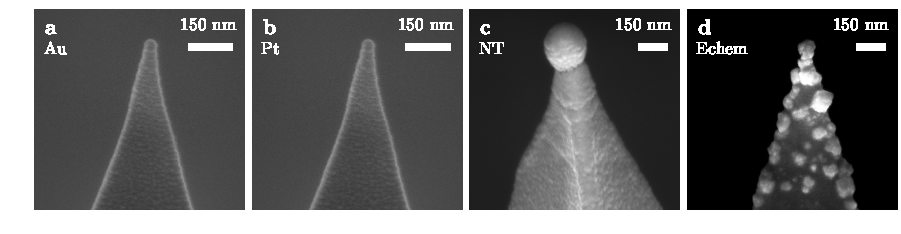
\includegraphics{figures/tip_sems}
\caption[SEM images of sharp and spherical metal tips studied using hyperspectral imaging]{\textbf{SEM images of sharp and spherical metal tips studied using hyperspectral imaging.} Tips are  (a) a sharp Au AFM tip, (b) a sharp Pt AFM tip, (c) a NT Au-coated spherical AFM tip and (d) an electrochemically deposited AuNP-on-Pt AFM tip.}
\label{fig:tip_sems}
\vspace{-10pt}
\end{figure}

% Lead into hyperspectral images and tip comparisons
To effectively {\color{red}investigate/understand} the plasmonics of nanostructured tips, hyperspectral images are taken of four different AFM probes. AFM tips studied are Au- and Pt-coated standard AFM probes (BudgetSensors), \SI{300}{nm} Au-coated NanoTools B150 AFM probes {\color{red}(spherical tips)} \cite{savage2012} and AuNP-on-Pt AFM probes, fabricated in-house using electrochemical deposition \cite{sanders2014}. SEM images of these tips are show in Fig.~{\ref{fig:tip_sems}}.
Fabricated tips are pre-treated where possible prior to use with ambient air plasma and/or piranha solution to remove organic surface residue and, in some cases, smooth surface roughness.
% is the cleaning necessary since this isn't a sub-nm contact paper?

\begin{figure}[bt]
\centering
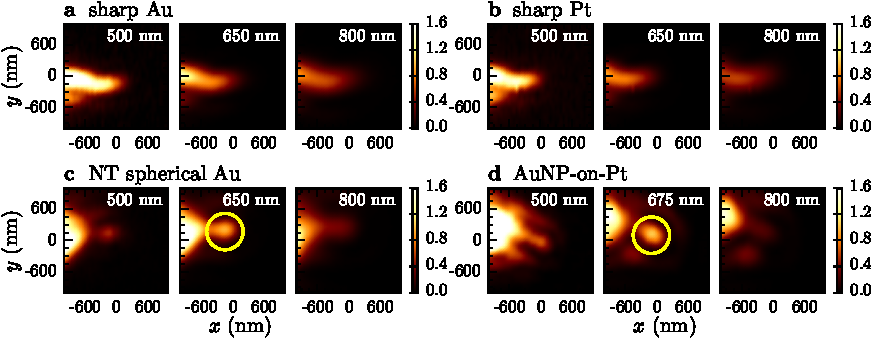
\includegraphics{figures/hyperspectral_tip_comparison}
\caption[Hyperspectral images of sharp and spherical metal tips at wavelengths of interest]{\textbf{Hyperspectral images of sharp and spherical metal tips at wavelengths of interest.} Images are of (a) a sharp Au tip, (b) a sharp Pt tip, (c) a NanoTools Au-coated spherical tip and (d) an electrochemically deposited AuNP-on-Pt tip. Collection polarisation is along the tip axis. Colour maps between slices all have the same normalisation.
Scattering from the spherical apex is clearly seen in the hyperspectral images of between 600-\SI{700}{nm}.}
\label{fig:hyperspectral_tip_comparison}
\vspace{-5pt}
\end{figure}

% Brief description of hyperspectral results
Comparisons between spherical- and sharp-tipped probes using hyperspectral image slices (Fig.~\ref{fig:hyperspectral_tip_comparison}) show that spherical tips exhibit a characteristic red (600-\SI{700}{nm}) scatter, delocalised from the bulk tip. No similar localised scattering is seen for sharp Au or Pt tips in the visible spectrum, which have an overall weaker optical response. This delocalised apex scatter is typically seen much clearer than when observed in conventional widefield microscopy (Fig.~\ref{fig:experiment}{\color{red}(inset)/(a)}). SEM images confirm that this glow occurs only with spherical tip shapes, or when a AuNP is securely attached at the tip apex with a sufficiently small neck joint.

% Show apex spectra comparison here
\begin{figure}[bt]
\centering
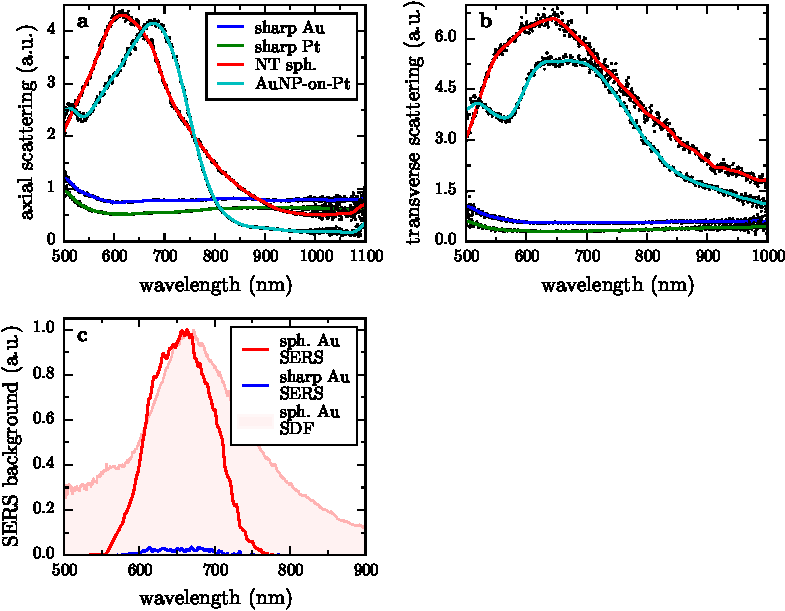
\includegraphics{figures/apex_spectra_comparison}
\caption[Apex spectra of sharp and spherical metal tips]{\textbf{Apex spectra of sharp and spherical metal tips.} Spectra are extracted from the hyperspectral images in Fig.~\ref{fig:hyperspectral_tip_comparison} by integrating pixels around the apex region. A clear resonance at \SI{630}{nm} is observed with spherical tips in both polarisations. The axial/longitudinal tip resonance is blueshifted \SI{20}{nm} from the longer transverse resonance. Sharp metallic tips show comparatively flat spectra.}
\label{fig:apex_spectra}
\vspace{-5pt}
\end{figure}

% Apex spectra comparisons
Spectra of tip apices clearly show a structural resonance excited in spherical tips with no obvious resonances present in sharp tips (Fig.~\ref{fig:apex_spectra}). Apex scatter of spherical tips is strong enough relative to bulk of the tip that it is easily observable with conventional dark-field microscopy  superimposed onto the bulk background scatter (Fig.~\ref{fig:lsp_confirmation}). These scattering resonances around \SI{630}{nm} are reliably present in all spherical-tipped probes, both vacuum-processed and electrochemically deposited AuNP-on-Pt, and are attributed to direct LSP excitation. The response of sharp Au tips show no plasmonic features while the slow rise in scattering towards the NIR is consistent with lightning rod scattering \cite{zhang2009}.

% Validation of SDF spectra and plasmonic observations
\begin{figure}[bt]
\centering
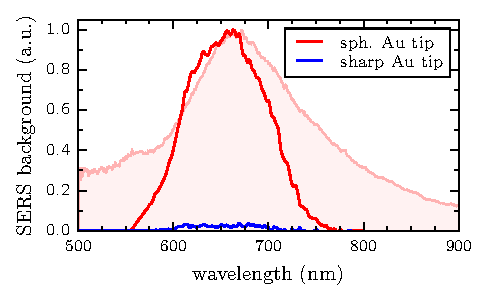
\includegraphics{figures/lsp_confirmation}
\caption[Integrated inelastic electron fluorescence measurements of both a sharp and spherical Au tip]{\textbf{Integrated inelastic electron fluorescence measurements of both a sharp and spherical Au tip.} Fluorescence spectra are acquired using tuneable, single wavelength spectroscopy with integrated spectra plotted as a function of excitation wavelength. The background spectrum is the supercontinuum dark-field scattering spectrum of the spherical Au tip apex, as measured using hyperspectral imaging. Agreement between the fluorescence (near-field) and dark-field scattering (far-field) spectra confirms resonant near-field enhancement as a \gls{lsp} excitation. Sharp Au tips show no such resonance in either the near-field or far-field.}
\label{fig:lsp_confirmation}
\vspace{-5pt}
\end{figure}

Tuneable single wavelength spectroscopy (fluorescence/Raman spectroscopy) is used to confirm that the resonance is indeed a LSP by showing that the near-field is resonantly enhanced \cite{}. Weak near-field processes such as fluorescence and Raman scattering can be plasmonically enhanced and therefore detectable in the far-field. By tuning the laser wavelength and corresponding long-pass filter cut-off wavelength the plasmonic enhancement of near-field processes can be directly observed (Fig.~\ref{fig:lsp_confirmation}). Summation of the scattering counts at each excitation wavelength shows a distinct peak around the scattering resonance from Fig.~\ref{fig:apex_spectra}, confirming it as a LSP resonance.
Further, confirmation comes from direct observation of plasmon coupling between spherical tips, previously reported \cite{savage2012}.

% Differences between types of spherical tips
Surprisingly, the overall disorder and parasitic edge AuNP nucleation on AuNP-on-Pt only minimally effects the overall optical response from the apex growth. Moreso, the AuNP-on-Pt structure behaves very similar to the Au-coated diamond-like-carbon spherical tip, likely because the \SI{50}{nm} coating thickness is greater than the skin depth \cite{stockman2011, huber2014}. Plasmons therefore see both as solid Au spheres. Differences arise due to the differences in neck material with Au-Pt and Au-Au neck boundaries.

\FloatBarrier
\section{Discussion}

The plasmon modes of a spherical tip are not so different from those of a {\color{red}sphere/AuNP} and can be explained accordingly. Like AuNP plasmons, spherical tip LSPs are specifically \emph{radiative} antenna modes, those that can efficiently couple far-field light with the near-field without the need for  momentum matching due to SPP dispersion. {\color{red}On the contrary, LSPs have constant dispersion and require excitation at the resonant wavelength.}  Radiative antenna LSP modes form only when two close dielectric surfaces surround a metallic particle, allowing the formation of confined multipolar charge oscillations. The resonance wavelength of these modes depends heavily on the spacing between each of the metal/dielectric interfaces, as is observed in the polarisation anisotropy in rod-like or ellipsoidal nanoparticle spectra \cite{mock2002, kuwata2003}.

Spherical metal tips retain some of the back hemisphere around the connection to the base tip apex, known as the neck region, allowing the spherical apex surface to sustain (multipolar) antenna-like plasmons. Sharp tips do not have this back surface, hence cannot support such resonances.
Their metal-dielectric surface still, however, supports the launching of SPPs in the near-field if the {\color{red}coupling/launching} conditions are satisfied. The requirement for evanescent coupling means that while a sharp tip can be considered an optical antenna its supported modes are considered as \emph{evanescent} or \emph{near-field} modes rather than \emph{radiative} antenna modes. 

\FloatBarrier
%\subsection{Simulated Near-Field of Spherical Tips and Simple Analytical Modelling}

\begin{figure}[bt]
\centering
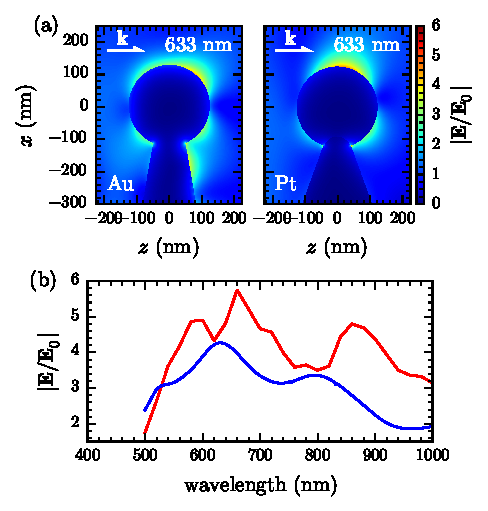
\includegraphics{figures/spherical_tip_near_fields}
\caption[Numerical simulations of the field enhancement around a spherical Au tip]{\textbf{Numerical simulations of the field enhancement around a spherical Au tip.} (a) Numerical simulations of the near-field around a spherical Au tip and a AuNP-on-Pt tips, both with \SI{250}{nm} sphere diameters and \SI{100}{nm} neck diameters. (b) Field enhancement as a function of wavelength, calculated as the summation of the near-fields are shown in (a).}
\label{fig:spherical_tip_near_fields}
\end{figure}

% Near-field simulations and identification of mode charge distributions
Numerical simulations of the near-field around spherical tips, computed using BEMAX, show the plasmon modes of a \SI{250}{nm} spherical Au tip. The modes of Au and AuNP-on-Pt spherical tips with \SI{100}{nm} neck diameters are shown in Fig.~\ref{fig:spherical_tip_near_fields}(a). Corresponding field enhancement spectra, calculated as the sum of the near-field, are shown in Fig.~\ref{fig:spherical_tip_near_fields}(b). A neck width of 0.4 times the sphere diameter (\SI{100}{nm} in this case) is used to match with typical experimental structures. Clear plasmon resonances for both Au and AuNP-on-Pt are found in the calculations with the dominant mode between 600--\SI{700}{nm} agreeing with experimental far-field scattering. From the near-field it is clear that the 600--\SI{700}{nm} SPR in spherical Au tips has a quadrupolar distribution while the longer wavelength dipolar mode exists between 850-\SI{1000}{nm}. Other resonances in the near-field, such as those localised solely around the neck crevices, do not fulfil the antenna conditions and therefore do not couple with light. The dipolar mode shows a strong field at the apex but little field around the rear suggesting it should also be significantly reduced in intensity or even dark, explaining why it is not optically observable.

Replacing the Au base tip with a Pt tip replicates the electrochemically-deposited AuNP-on-Pt tips and changes the mode structure. The mode around \SI{630}{nm} becomes more dipolar in its near-field distribution.

The dependence of the modes and field enhancement on the width of the neck is investigated by widening the neck region until the back surface of the spherical tip disappears. The tip structure therefore transitions from a AuNP until the morphology resembles that of a sharp tip, albeit with a large radius of curvature. The plasmonic contribution of the spherical tip is therefore able to be quantified independent of the lightning rod contribution, which remains constant between all geometries.

\begin{figure}[bt]
\centering
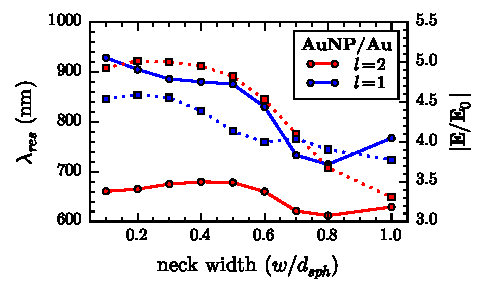
\includegraphics{figures/spherical_tip_neck_size_dependence}
\caption[Resonant wavelength and field enhancement dependence on the neck width]{\textbf{Resonant wavelength and field enhancement dependence on the neck width.} The resonant wavelength (solid lines) and field enhancement (dashed lines) are plotted for the dipolar (blue) and quadrupolar (red) modes of spherical Au and AuNP-on-Pt tips.}
\label{fig:neck_size_dependence}
\end{figure}

Increases in the neck diameter cause a strong blueshift of the dipolar mode from \SI{1000}{nm} to \SI{850}{nm} (Fig.~\ref{fig:neck_size_dependence}). The quadrupolar mode is far less susceptible to changes in the neck region and therefore does not shift. This explains the robustness of the observed spherical tip plasmon regardless of tip morphology.

The importance of this change is that the largest fields are located at the apex surface along the tip axis, meaning that any surface sees the maximum possible field enhancement. In the case with a spherical Au tip the near-field distribution is quadrupolar which means that the region of maximum field enhancement can never reach the area underneath the AFM tip.

%\subsection{Implications}

% Focus on the implications of tip plasmons first, then on the use of appropriate spectroscopy
From the presented results we can say that it is important to first consider what plasmons might exist in a particular geometry and the illumination conditions/polarisations required to excite the mode. The existence of radiatively coupled LSPs opens up more experimental geometries using only far-field light, such as the side illumination configuration. If only near-field SPPs exist then evanescent wave coupling must be employed.
%If only near-field SPPs exist then it is necessary to employ evanescent wave coupling.
Regardless of the plasmonics and illumination, the sharpness of the probe will always play a role due to the non-resonant lightning rod effect. By understanding the underlying plasmon modes and the required excitation conditions, combined with pre-characterisation of tips, the field enhancement of tip-based nano-spectroscopy can be {\color{red}optimised/maximised}. Through correct nanostructuring of the apex, modes can be tuned across the visible spectrum and brought into resonance with available laser wavelengths.
% Why optics needs to be considered before drawing conclusions from spectra
When characterising probes it is necessary to consider an applicable spectroscopy technique. Spectral peaks {\color{red}or shifts} from tips observed using wide-field techniques cannot be guaranteed to be localised to the apex. By utilising hyperspectral confocal imaging, with its higher resolution, radiative antenna modes can be locally probed. Furthermore, tuneable single wavelength spectroscopy identifies only features that enhance near-field processes whilst rejecting all other reflections or back-scattering.
% Why a 630 nm optically excitable tip mode is useful
A significant result of pre-characterising tips is the direct observation that nanostructuring a tip with a sphere gains the tip a robust, far-field coupled apex plasmon around \SI{633}{nm}. {\color{red}The field enhancement on resonance is sufficient enough for TERS measurements \cite{umakoshi2012, sanders2014}}.
% Analytical equations also suggest that a plasmonic enhancement is far stronger than the lightning rod effect \cite{Goncharenko2006}. For this reason nanostructured tips have the potential to outperform sharp tips, to which even the sharpest tips have a limit to field enhancement set by the onset of nonlocal effects \cite{Wiener2012}.
This both relieves the requirement of near-field excitation and allows one to use readily available HeNe or diode lasers.

% Implementing gap modes with these structures
As is typically employed in SERS, the degree of {\color{red}confinement/localisation} of hotspots is increased through the formation of gap modes between two plasmonic surfaces, increasing the local field enhancement. If the gap modes comprise of at least coupled antenna mode the gap is accessible from the far-field. This allows plasmon coupling to be directly observed experimentally and monitored as a function of gap size \cite{savage2012}. %The optimal wavelength for near-field excitation of a gap can then be experimentally determined as a function of gap size rather than guessed.
In such cases where the lateral width of the gap mode \cite{romero2006} is small, as is typically the case with nm-scale gaps, the plasmonic contribution will outweigh a lightning rod contribution \cite{}, hence spherical tips have the capability of outperforming much sharper tips. Spherical tips are particularly optimised for use in this configuration since its coupled mode becomes resonant with \SI{785}{nm} laser light typically found on Raman microscopes for gaps below \SI{2}{nm} \cite{}. Sharp tip TERS tends to use a \SI{488}{nm} wavelength, likely due to the intrinsic increase in bluer light Rayleigh scattering off the sharp point.

%Furthermore, the addition of amplification or filtering to remove background scattering is no longer necessary when using antenna probes \cite{}.

% Comparison with NPoM systems that use AuNP plasmons for SERS
The use of radiative antenna modes in nanostructured tips bridges the gap between SERS and TERS structures. Some of the largest enhancement factors recently measured in plasmonic systems originate from antenna modes in NPs coupled with the charge distribution of their image in a mirror \cite{mertens2013, taylor2014}. These systems repeatedly produce {\color{red}Raman/field/intensity} enhancement factors of up to $10^7$, much like tips, with mode volumes of coupled plasmons on the nm-scale. These systems demonstrate that a plasmonic gap mode can exhibit large field enhancement without requiring contribution from the lightning rod effect. However, the static nature of the NPoM geometry lacks the ability to chemically map a surface. By coupling plasmons in spherical tips with their mirrored image charge a surface could be dynamically mapped with a potentially large field enhancement.

%\section{Conclusions}

In conclusion, we show that localised surface plasmons can be clearly observed in extended nanostructures using a scanning-confocal hyperspectral imaging in a supercontinuum dark-field microscope. This enables plasmon-dependent applications, such as TERS, to pre-screen nanostructured tips to better improve the reliability and reproducibility of such techniques. Using this technique, the optical/scattering response of spherical-tipped AFM probes is shown to exhibit resonances not present in standard metallic AFM probes. Observed resonances correspond to antenna modes of the system, those which couple readily with light without the need for momentum matching. These modes determine what plasmonic phenomena are able to be experimentally observed, hence spherical tips can be used to dynamically investigate plasmonics.
\end{document}